\documentclass[12pt]{article}
\usepackage{amsmath,amssymb,amsthm}
\usepackage{graphicx,mathabx}
\usepackage{xcolor}
\usepackage{tikz}
\usepackage{placeins}
\usepackage{lipsum}
\usepackage[shortlabels]{enumitem}
\begin{document}
\title{TCSS 343 - Week 3}
\author{Jake McKenzie}
\maketitle
\noindent\centerline{\textbf{Divide and Conquer}}\\\\\\\\\\\\\\\\
\begin{center}
    ``Common misconception that \textit{fun} is relaxing. \\If it is, you’re not doing it right." \\$\cdots$\\ Iain Banks
\end{center}
\begin{center}
    ``Writing is nature's way of letting you know how sloppy your thinking is." \\
    $\dots$\\
    Guindon
\end{center}
\begin{center}
    ``Do those things that incline you toward the big questions, and avoid the things that would reduce you and make you trivial." \\$\cdots$\\ George Saunders 
\end{center}
\newpage
0. Use the master method to solve the following recurrences. If the master method does not apply indicate that it does not.
\begin{enumerate}
    \item[I)]$T(n) = 7T(\frac{n}{7}) + O(n)$
    \item[II)]$T(n) = 5T(\frac{n}{3}) + O(n)$
    \item[III)]$T(n) = 3T(\frac{2}{n}) + O(1)$
    \item[IV)]$T(n) = 16T(\frac{n}{4}) + O(n^3)$
    \item[V)]$T(n) = 4T(\frac{n}{9}) + O(n \log{n})$
    \item[VI)]$T(n) = T(\frac{n}{9}) + O(\sqrt{n})$
    \item[VII)]$T(n) = 7T(\frac{n}{2}) + O(n^2)$
    \item[VIII)]$T(n) = 4T(\frac{n}{2}) + O(16^{\log{n}})$
    \item[IX)]$T(n) = 2T(n) + O(n^3)$
    \item[X)]$T(n) = 2T(\frac{n}{3}) + O(n^{-\log{n}})$
    \item[XI)]$T(n) = 2T(\frac{n}{2}) + O(n^{0.51})$
\end{enumerate}
\newpage
1. Consider the problem of searching an element x in an array ‘arr[]’ of size $n$. The problem can be solved in $O(\log{n})$ time if:\\
\begin{enumerate}
    \item[I)]Array is sorted
    \item[II)]Array is sorted and rotated by $k$. $k$ is given to you and $k \leq n$
    \item[III)]Array is sorted and rotated by $k$. $k$ is NOT given to you and $k \leq n$
    \item[IV)]Array is not sorted
\end{enumerate}
\begin{enumerate}
    \item[a)]I
    \item[b)]I and II
    \item[c)]I,II and III
    \item[d)]I,II,III and IV
\end{enumerate}
2. What is the probability that a number is composite numbers in first 50 natural numbers inclusive? (hint: 1 is neither composite nor prime and composite). (I've seen this question in pools of interview questions for algorithms) 
\begin{enumerate}
    \item[a)]$0.58$
    \item[b)]$0.62$
    \item[c)]$0.68$
    \item[d)]$0.72$
\end{enumerate}
\newpage
3. Solve the following recurrence: $T(n) = T(\frac{6n}{7}) + T(\frac{n}{7})  + O(n)$. The master method cannot be used on this one. Use the tree method or repeated substition to find the runtime.
\newpage
\noindent 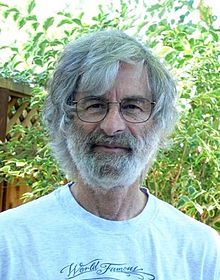
\includegraphics[scale = 0.5]{lamport.jpg}
Thinking doesn't guarantee that we won't make mistakes. But not thinking guarantees that we will. $\sim$ Leslie Lamport (turing award winnder, both devised important algorithms and ways of formal modeling)\\\\
4. \textbf{Preferably by using your notes, write down a formal specification for quicksort}. Formal specifications are important, they give us the language to describe subtle problems that you can't get from simply writing code. When students hear ``specifications" they typically panic. You have to learn and use these funny symbols and such, but if you don't get it right that's okay. The world isn't going to come crashing down if you don't do get it perfectly right but please try.  
\newpage
\noindent 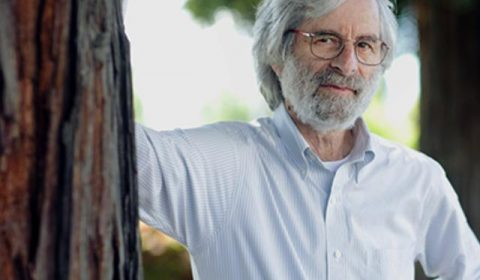
\includegraphics[scale = 0.5]{lamport2.jpg}
Writing formal specifications won't catch coding errors or bugs, but it will catch algorithm errors. $\sim$ Leslie Lamport (the guy from the previous page)
\\\\5. You typically write specifications while thinking about the problem, before you write code. I'm assuming you probably wrote a recursive specification for quicksort on the previous page. If you didn't, great you're done you can move on. \textbf{If you did write a recursive specification for quicksort, please now attempt to write a non-recursive specification for quicksort}. This is more challenging but please, please try to do so. It requires more thought but thinking is a really good idea; don't trust anyone who tells you otherwise. \textbf{Come up with one reason why you think it's a good idea to write a spec}.
\newpage
\noindent A really important algorithm that's used on the backend that you've probably never heard of is known as \textit{rotate}. It's is a fundamental tool used behind the scenes in all sorts of computer graphics from updating frame buffers on embedded devices to websites. We can even give a formal mathematical \textbf{specification}:  \\\\
\centerline{A permutation of $n$ elements by $k$ where $k\geq 0$}:
$$(k\mod{n},k+1\mod{n},\dots,k+n-1\mod{n},k+n-1\mod{n})$$
Mathematical specifications can be nice compact ways of specifying algorithms when we can find them, but this isn't always possible. My favourite way that I've seen this implemented is the Gries-Mills Block Swapping algorithm which is an inplace algorithm:\\\\
\noindent 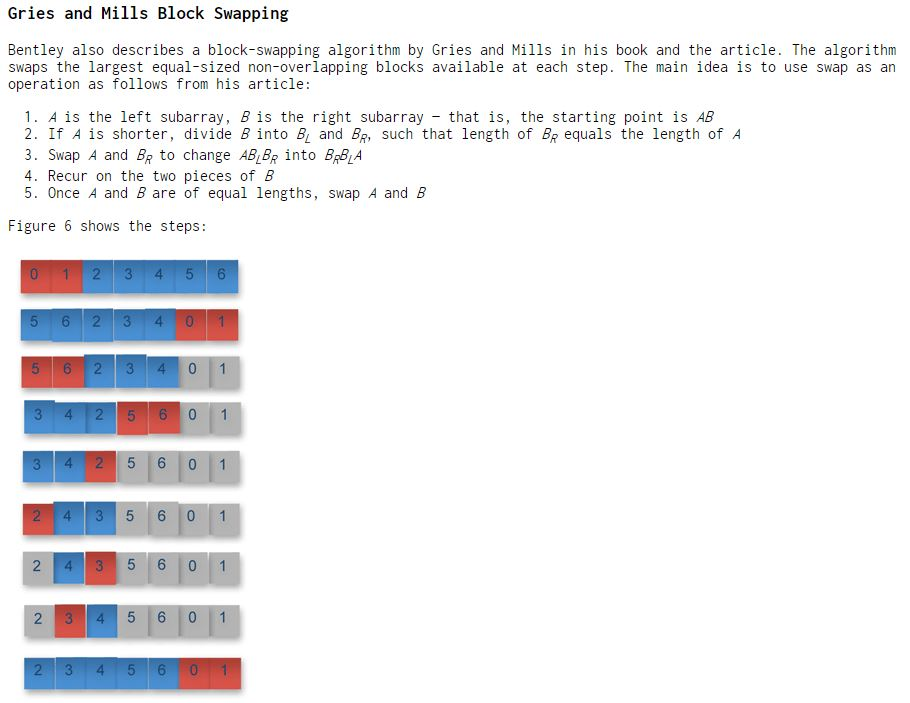
\includegraphics[scale = 0.65]{griesmills.jpg}
\newpage
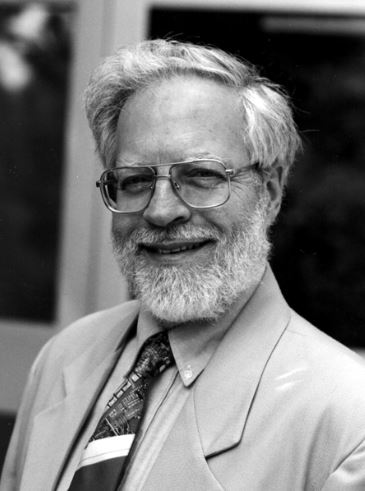
\includegraphics[scale = 0.25]{gries.jpg}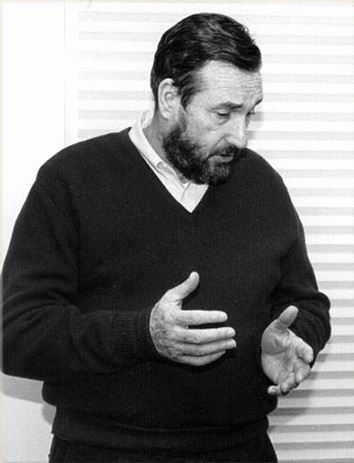
\includegraphics[scale = 0.25]{mills.jpg}
6. Can you write down an algorithm that does what is described on the last page, it need not be Gries-Mills'(pictured $\leftarrow$) block swapping algorithm, that attempts to do \textit{rotate}?
\newpage

\end{document}